\documentclass[Cal1Spr16Lectures.tex]{subfiles}

\begin{document}

\section[Week 3]{Week 3: 1-5 February}

% % %
\subsection[2.6 Continuity]{\S2.6 Continuity}
% % %

% % %
\begin{frame}{\S2.6 Continuity}\footnotesize
Informally, a function $f$ is ``continuous at $x=a$" means for $x$-values anywhere close enough to $a$ the graph can be drawn without lifting a pencil.  In other words, no holes, breaks, asymptotes, etc.
\begin{dfn} A function $f$ is {\bf continuous} at $a$ means
\[\lim_{x \to a} f(x)=f(a).\]  
If $f$ is not continuous at $a$, then $a$ is a {\bf point of discontinuity}. \end{dfn}
\end{frame}

% % %
\subsubsection{Continuity Checklist}
% % %

% % %
\begin{frame}{\small Continuity Checklist}\footnotesize
In order to claim something is continuous, you must verify all three:
\begin{itemize}
\item[1.] \alert{$f(a)$ is defined} (i.e., $a$ is in the domain of $f$ -- no holes, asymptotes).
\item[2.] \alert{$\displaystyle\lim_{x \to a} f(x)$ exists.}  You must check both sides and make sure they equal the same number.
\item[3.] \alert{$\displaystyle\lim_{x \to a} f(x) = f(a)$} (i.e., the value of $f$ equals the limit of $f$ at $a$).  
\begin{que} What is an example of a function that satisfies this condition? \end{que}
\end{itemize}
\end{frame}

% % %
\begin{frame}\footnotesize
\begin{columns}[T]
	\begin{column}{.65\textwidth}
		\begin{ex} \begin{itemize}
		\item Where are the points of discontinuity of the function below?  
		\item Which aspects of the checklist fail?
		\end{itemize}
		\centering{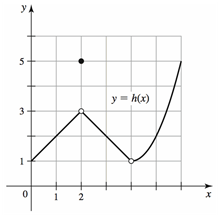
\includegraphics[scale=0.72]{pictures/Ch2Sect2_Exer7}}
		\end{ex}
	\end{column}
	\begin{column}{.4\textwidth}
	\vspace{8pc}
		recall (Continuity Checklist):
			\vspace{-1pc}
			\begin{itemize}
			\item[1.] function is defined
			\item[2.] the two-sided limit exists
			\item[3.] 2.\;=\;1.
			\end{itemize}
	\end{column}
\end{columns}
\end{frame}

% % %
\subsubsection{Continuity Rules}
% % %

% % %
\begin{frame}{\small Continuity Rules}
If $f$ and $g$ are continuous at $a$, then the following functions are also continuous at $a$.  Assume $c$ is a constant and $n>0$ is an integer.
\begin{itemize}
\item[1.] $f+g$
\item[2.] $f-g$
\item[3.] $cf$
\item[4.] $fg$
\item[5.] $\frac{f}{g}$, provided $g(a)\ne 0$
\item[6.] $[f(x)]^n$
\end{itemize}
\end{frame}

% % %
\begin{frame}
From the rules above, we can deduce:
\begin{itemize}
\item[1.] Polynomials are continuous for all $x=a$.
\item[2.] Rational functions are continuous at all $x=a$ except for the points where the denominator is zero.  
\item[3.] If $g$ is continuous at $a$ and $f$ is continuous at $g(a)$, then the composite function $f \circ g$ is continuous at $a$.
\end{itemize}
\end{frame}

% % %
\subsubsection{Continuity on an Interval}
% % %

% % %
\begin{frame}{\small Continuity on an Interval}\footnotesize 
Consider the cases where $f$ is not defined past a certain point. 
\begin{dfn}
A function $f$ is {\bf continuous from the left} (or {\bf left-continuous}) at $a$ means
\[\lim_{x \to a^-} f(x)=f(a);\]
a function $f$ is {\bf continuous from the right} (or {\bf right-continuous}) at $a$ means
\[\lim_{x \to a^+} f(x)=f(a).\]
\end{dfn}
\end{frame}

% % %
\begin{frame}
\begin{dfn} A function $f$ is {\bf continuous on an interval $I$} means it is continuous at all points of $I$. \end{dfn}  
Notation: Intervals are usually written 
\[\left[a,b\right],\;\left(a,b\right],\;\left[a,b\right),\text{ or }\left(a,b\right).\]
When $I$ contains its endpoints, ``continuity on $I$" means continuous from the right or left at the endpoints.
\end{frame}

% % %
\begin{frame}
\begin{ex}Let $f(x)=\begin{cases}
	x^3+4x+1 & \text{if}\ x \leq 0 \\
	2x^3 & \text{if}\ x>0.
	\end{cases}$
\begin{itemize}
\item[1.] Use the continuity checklist to show that $f$ is not continuous at 0.
\item[2.] Is $f$ continuous from the left or right at 0?
\item[3.] State the interval(s) of continuity.
\end{itemize}
\end{ex}
\end{frame}

% % %
\subsubsection{Continuity of Functions with Roots}
% % %

% % %
\begin{frame}{\small Continuity of Functions with Roots}{}
{\small (assuming $m$ and $n$ are positive integers and $\textstyle\frac{n}{m}$ is in lowest terms)}
\begin{itemize}
\item If $m$ is odd, then $[f(x)]^{\frac{n}{m}}$ is continuous at all points at which $f$ is continuous.
\item If $m$ is even, then $[f(x)]^{\frac{n}{m}}$ is continuous at all points $a$ at which $f$ is continuous \alert{and $f(a)\geq 0$}.
\end{itemize}
\begin{que}  Where is $f(x)=\sqrt[4]{4-x^2}$ continuous?\end{que}
\end{frame}

% % %
\subsubsection{Continuity of Transcendental Functions}
% % %

% % %
\begin{frame}{\small Continuity of Transcendental Functions}
\footnotesize
{\bf Trig Functions:} The basic trig functions are all continuous at all points \alert{IN THEIR DOMAIN}.  Note there are points of discontinuity where the functions are not defined -- for example, $\tan x$ has asymptotes everywhere that $\cos x=0$.  

\vspace{1pc}
{\bf Exponential Functions:}  The exponential functions $b^x$ and $e^x$ are continuous on all points of their domains.

\vspace{1pc}
{\bf Inverse Functions:}  If a continuous function $f$ has an inverse on an interval $I$ (meaning if $x\in I$ then $f^{-1}(y)$ passes the vertical line test), then its inverse $f^{-1}$ is continuous on the interval $J$, which is defined as all the numbers $f(x)$, given $x$ is in $I$.
\end{frame}

% % %
\subsubsection{Intermediate Value Theorem (IVT)}
% % % 

% % %
\begin{frame}{\small Intermediate Value Theorem (IVT)}
\begin{thm}[Intermediate Value Theorem] Suppose \alert{$f$ is continuous on the interval $[a,b]$} and $L$ is a number satisfying
\[f(a)<L<f(b)\quad\text{or}\quad f(b)<L<f(a).\]  
Then there is at least one number $c\in (a,b)$, i.e., $a<c<b$, satisfying 
\[f(c)=L.\] 
\end{thm}
\end{frame}

% % %
\begin{frame}
\begin{ex} Let $f(x)=-x^5-4x^2+2\sqrt{x}+5.$  Use IVT to show that $f$ has a root (i.e., $f(x)=0$ has a solution) in the interval $(0,3)$. \end{ex}
\end{frame}

% % %
\begin{frame}
\begin{exe} Which of the following functions is continuous for all real values of $x$?
\begin{itemize}
\item[(A)\;] $f(x)=\frac{x^2}{2x+1}$
\item[(B)\;] $g(x)=\sqrt{3x^2-2}$
\item[(C)\;] $h(x)=\frac{5x}{|x^8-1|}$
\item[(D)\;] $j(x)=\frac{5x}{x^8+1}$
\end{itemize}
\end{exe}
\end{frame}

% % %
\subsubsection{Book Problems}
\begin{frame}
\begin{block}{2.6 Book Problems} 9-25 (odds), 35-45 (odds), 59, 61, 63, 83, 85 \end{block} 
\end{frame}

% % %
\subsection[2.7 Precise Definitions of Limits]{\S 2.7 Precise Definitions of Limits}
% % %

% % %
\begin{frame}{\S 2.7 Precise Definitions of Limits}\small
So far in our dealings with limits, we have used informal terms such as ``sufficiently close" and ``arbitrarily large".  Now we will formalize what these terms mean mathematically.

\vspace{1pc}
\textbf{Recall:} $|f(x)-L|$ and $|x-a|$ refer to the distances between $f(x)$ and $L$ and between $x$ and $a$.

\vspace{1pc}
Also, recall that when we worked informally with limits, we wanted $x$ to approach $a$, \alert{but not necessarily equal $a$}.  Likewise, we wanted $f$ to get arbitrarily close to $L$, but not necessarily equal $L$.
\end{frame}

% % %
\begin{frame}\footnotesize
\begin{dfn}
Assume that $f(x)$ exists for all $x$ in some open interval (open means: neither of the endpoints not included) containing $a$, except possibly at $a$.  \textbf{``The limit of $f(x)$ as $x$ approaches $a$ is $L$"}, i.e.,
\[\lim_{x \to a}f(x)=L,\]
means \textbf{for any $\epsilon > 0$ there exists $\delta > 0$ such that} 
\[|f(x)-L|<\epsilon \quad \textbf{whenever} \quad 0<|x-a|<\delta.\]
\end{dfn}
\begin{que}
Why $0<|x-a|$ but not for $|f(x)-L|$?
\end{que}

\end{frame}

% % %
\subsubsection{$\epsilon$ and $\delta$}
% % %

% % %
\begin{frame}{\small $\epsilon$ and $\delta$}\small
When we worked informally with limits, we saw $f(x)$ get closer and closer to $L$ as $x$ got closer and closer to $a$. 

\begin{que} If we want the distance between $f(x)$ and $L$ to be less than $1$, how close does $x$ have to be to $a$? What if we want $|f(x)-L|<0.5$?  $0.5$? $0.1$? $0.01$?  
\end{que}
\end{frame}

% % %
\subsubsection{Seeing $\epsilon$s and $\delta$s on a Graph}
% % %

% % %
\begin{frame}{\small Seeing $\epsilon$s and $\delta$s on a Graph}\footnotesize
\begin{ex}
\begin{columns}[T]
	\begin{column}{.36\textwidth}
		\centering{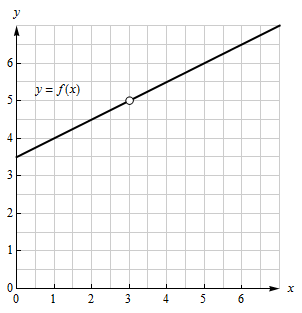
\includegraphics[scale=0.55]{pictures/Fig2_57}}
	\end{column}
	\begin{column}{.5\textwidth}
		Using the graph, for each $\epsilon >0$, determine a value of $\delta>0$ to satisfy the statement 
		\begin{multline*}|f(x)-5|<\epsilon\quad\text{whenever} \\
			0<|x-3|<\delta.\end{multline*}  
		\vspace{-1.5pc}
		\begin{itemize}
		\item[(a) ] $\epsilon=1$ 
		\item[(b) ] $\epsilon=0.5$.
		\end{itemize}
	\end{column}
\end{columns}
\end{ex}
\end{frame} 

% % %
\begin{frame}{\small Seeing $\epsilon$s and $\delta$s on a Graph, cont.}\footnotesize
When $\epsilon=1$:
\vspace{-0.25pc}
\begin{columns}
\begin{column}{.36\textwidth}
\begin{block}
\centering{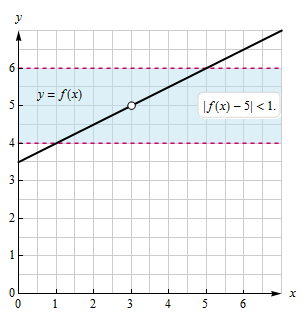
\includegraphics[scale=0.45]{pictures/Fig2_57a}}
\end{block}
\end{column}
\begin{column}{.36\textwidth}
\begin{block}
\centering{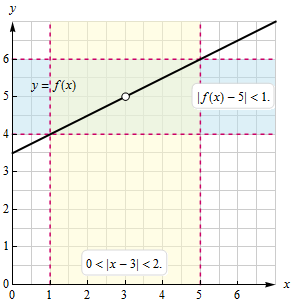
\includegraphics[scale=0.47]{pictures/Fig2_57b}}
\end{block}
\end{column}
\end{columns}
\vspace{-0.75pc}
\flushright $\dots\;\delta=2$
\end{frame}

% % %
\begin{frame}{\small Seeing $\epsilon$s and $\delta$s on a Graph, cont.}\footnotesize
When $\epsilon=0.5$:
\vspace{-0.25pc}
\begin{columns}
\begin{column}{.36\textwidth}
\begin{block}
\centering{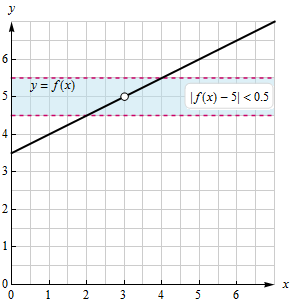
\includegraphics[scale=0.47]{pictures/Fig2_58}}
\end{block}
\end{column}
\begin{column}{.36\textwidth}
\begin{block}
\centering{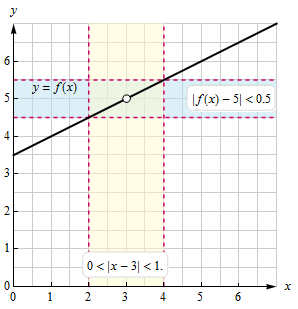
\includegraphics[scale=0.47]{pictures/Fig2_58a}}
\end{block}
\end{column}
\end{columns}
\vspace{-0.75pc}
\flushright $\dots\;\delta=1$
\end{frame}

% % %
\begin{frame}{}
The $\epsilon$s and $\delta$s give a way to visualize computing the limit, and prove it exists.  As the $\epsilon$s get smaller and smaller, we want there to always be a $\delta$.  In this example,
\[\lim_{x\to 3}f(x)=5.\]
\end{frame}

% % %
\begin{frame}\footnotesize
\begin{exe}
\vspace{0.75pc}
\begin{columns}[T]
	\begin{column}{.22\textwidth}
		\centering{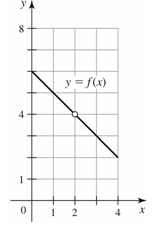
\includegraphics[scale=0.85]{pictures/Ch2Sect7_Exer10}}
	\end{column}
	\begin{column}{.6\textwidth}
		Using the graph, for each $\epsilon>0$, determine a value of $\delta>0$ to satisfy the statement
		\begin{multline*}|f(x)-4|<\epsilon\quad\text{whenever} \\
			0<|x-2|<\delta.\end{multline*}  
		\vspace{-1pc}
		\begin{itemize}
		\item[(a) ] $\epsilon=1$ 
		\item[(b) ] $\epsilon=0.5$.
		\end{itemize}
	\end{column}
\end{columns}
\end{exe}
\end{frame} 

% % %
\subsubsection{Finding a Symmetric Interval}
% % % 

% % %
\begin{frame}{\small Finding a Symmetric Interval}
\begin{que}When finding an interval $(a-\delta, a+\delta)$ around the point $a$, what happens if you compute two different $\delta$s?\end{que}  
{\bf Answer:}  To obtain a symmetric interval around $a$, use the smaller of the two $\delta$s as your distance around $a$.
\end{frame}

% % %
\begin{frame}\footnotesize
\begin{exe}
\vspace{0.75pc}
\begin{columns}[T]
	\begin{column}{.4\textwidth}
		\centering{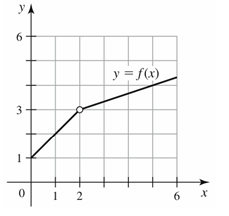
\includegraphics[scale=0.9]{pictures/Ch2Sect7_Exer15}}
	\end{column}
	\begin{column}{.55\textwidth}
		The graph of $f(x)$ shows 
		\[\lim_{x \to 2}f(x)=3.\] 
		For $\epsilon=1$, find the corresponding value of $\delta>0$ so that
		\begin{multline*}|f(x)-3|<\epsilon\quad\text{whenever} \\
			0<|x-2|<\delta.\end{multline*}  
	\end{column}
\end{columns}
\end{exe}
\end{frame}

% % %
\begin{frame}{}
\begin{exe} Let $f(x)=x^2-4$.  For $\epsilon=1$, find a value for $\delta>0$ so that 
\[|f(x)-12|<\epsilon \quad \text{whenever}\quad 0<|x-4|<\delta.\]
\end{exe}
In this example,  $\lim_{x \to 4}f(x)=12.$  
\end{frame}

% % %
\subsubsection{Book Problems}
% % %

% % %
\begin{frame}
\begin{block}{2.7 Book Problems} 1-7, 9-18 \end{block}
\end{frame}

% % %
\subsection[3.1 Introducing the Derivative]{\S Introducing the Derivative}
% % %

% % %
\begin{frame}{\S 3.1 Introducing the Derivative}{}
{\bf Recall from Ch 2:}  We said that the slope of the tangent line at a point is the limit of the slopes of the secant lines as the points get closer and closer.
\begin{itemize}
\item slope of secant line:  $\dfrac{f(x)-f(a)}{x-a}$\ (average rate of change) 
\item slope of tangent line:  $\lim_{x \to a} \frac{f(x)-f(a)}{x-a}$\ (instantaneous rate of change)
\end{itemize}
\end{frame}

% % %
\begin{frame}
\centering{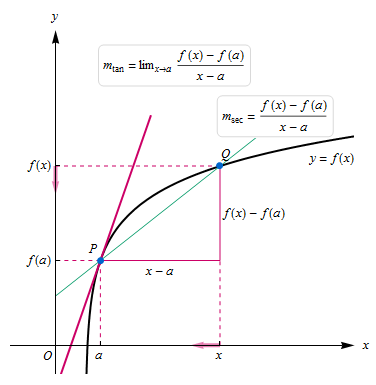
\includegraphics[scale=0.62]{pictures/lim}}
\end{frame}

% % %
\begin{frame}
\begin{exe} Use the relationship between secant lines and tangent lines, specifically the slope of the tangent line, to find the equation of a line tangent to the curve $f(x)=x^2+2x+2$ at the point $P=(1,5)$.
\end{exe}
\end{frame}

% % %
\begin{frame}{}
In the preceding exercise, we considered two points 
\vspace{-0.6pc}
\[P=\left(a,f(a)\right)\quad\text{and}\quad Q=\left(\alert{x},f(\alert{x})\right)\]
that were getting closer and closer together.

\vspace{2pc}
Instead of looking at the points approaching one another, we can also view this as the distance $h$ between the points approaching 0.  For 
\vspace{-0.5pc}
\[P=\left(a,f(a)\right)\quad\text{and}\quad Q=\left(\alert{a+h},f(\alert{a+h})\right),\]
\end{frame}

% % %
\begin{frame}
\begin{itemize}
\item slope of secant line:  
\[\frac{f(a+h)-f(a)}{(a+h)-a}= \dfrac{f(a+h)-f(a)}{h}\]
\item slope of tangent line:  
\[\lim_{h \to 0} \frac{f(a+h)-f(a)}{h}\]
\end{itemize}
\end{frame}

% % %
\begin{frame}
\centering{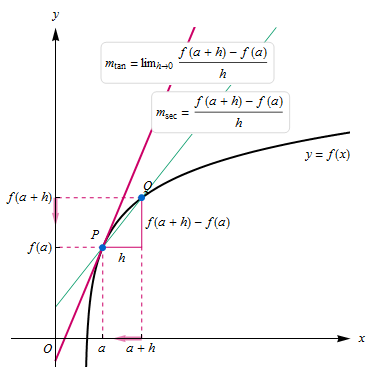
\includegraphics[scale=0.65]{pictures/limDef3_1}}
\end{frame}

% % %
\begin{frame}
\begin{exe} Find the equation of a line tangent to the curve $f(x)=x^2+2x+2$ at the point $P=(2,10)$. \end{exe}
\end{frame}

% % %
\subsubsection{Derivative Defined as a Function}
% % %

% % %
\begin{frame}{\small Derivative Defined as a Function}\footnotesize
The slope of the tangent line for the function $f$ is itself a function of $x$ (in other words, there is an expression where we can plug in any value $x=a$ and get the derivative at that point), called the derivative of $f$.
\begin{dfn} The {\bf derivative} of $f$ is the function 
\[f^{\prime}(x)=\lim_{h \to 0} \frac{f(x+h)-f(x)}{h},\]
provided the limit exists.  If $f^{\prime}(x)$ exists, we say $f$ is {\bf differentiable} at $x$.  If $f$ is differentiable at every point of an open interval $I$, we say that $f$ is differentiable on $I$. \end{dfn}
\end{frame}

% % %
\begin{frame}
\begin{exe} Use the definition of the derivative to find the derivative of the function $f(x)=x^2+2x+2$. \end{exe}
\end{frame}

% % %
\subsubsection{Leibniz Notation}
% % %

% % %
\begin{frame}{\small Leibniz Notation}
A standard notation for change involves the Greek letter $\Delta$. 
\[\frac{f(x+h)-f(x)}{h}=\frac{f(x+\Delta x)-f(x)}{\Delta x}=\frac{\Delta y}{\Delta x}.\]
Apply the limit:
\[f^{\prime}(x)=\lim_{\Delta x \to 0} \frac{f(x+\Delta x)-f(x)}{\Delta x}=\lim_{\Delta x \to 0} \frac{\Delta y}{\Delta x}=\alert{\frac{dy}{dx}}\]
\end{frame}

% % %
\subsubsection{Other Notation}
% % %

% % %
\begin{frame}{\small Other Notation}
The following are alternative ways of writing $f^{\prime}(x)$ (i.e., the derivative as a function of $x$):
\[\frac{dy}{dx}\qquad\frac{df}{dx} \qquad\frac{d}{dx}\left(f(x)\right) \qquad D_x (f(x)) \qquad y^{\prime}(x)\]
The following are ways to notate the derivative of $f$ evaluated at $x=a$:
\[f^{\prime}(a)\qquad y^{\prime}(a) \qquad \left. \frac{df}{dx} \right|_{x=a} \qquad \left. \frac{dy}{dx} \right|_{x=a}\]
\end{frame}

% % %
\begin{frame}
\begin{que}
Do the words ``derive" and ``differentiate" mean the same thing?
\end{que}
\end{frame}

% % %
\subsubsection{Graphing the Derivative}
% % %

% % %
\begin{frame}{\small Graphing the Derivative}
The graph of the derivative is the graph of the collection of slopes of tangent lines of a graph.  If you just have a graph (without an equation for the graph), the best you can do is approximate the graph of the derivative.
\end{frame}

% % %
\begin{frame}\footnotesize
\begin{ex}
\vspace{0.75pc}
\begin{columns}[T]
\begin{column}{0.45\textwidth}
	Simple checklist:
	\begin{itemize}
	\item[1.] Note where $f^{\prime}(x)=0$.
	\item[2.]  Note where $f^{\prime}(x)>0$.  (What does this look like?)
	\item[3.]  Note where $f^{\prime}(x)<0$.  (What does this look like?)
	\end{itemize}
\end{column}
\begin{column}{0.5\textwidth}	
	\centering{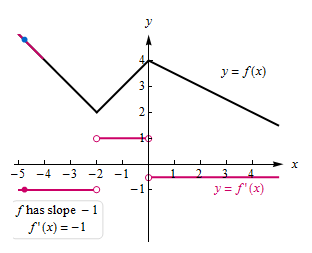
\includegraphics[scale=0.63]{pictures/graphDeriv3_1}}
\end{column}
\end{columns}
\end{ex}	
\end{frame}

% % %
\subsubsection{Differentiability vs. Continuity}
% % %

% % %
\begin{frame}{\small Differentiability vs. Continuity}
Key points about the relationship between differentiability and continuity:
\begin{itemize}
\item If $f$ is differentiable at $a$, then $f$ is continuous at $a$.
\item If $f$ is not continuous at $a$, then $f$ is not differentiable at $a$.
\item $f$ can be continuous at $a$, but not differentiable at $a$.
\end{itemize}
\end{frame}

% % %
\begin{frame}{}
A function $f$ is \alert{not} differentiable at $a$ if at least one of the following conditions holds:
\begin{itemize}
\item[1.] $f$ is not continuous at $a$.
\item[2.] $f$ has a corner at $a$.  
\begin{que} Why does this make $f$ not differentiable? \end{que}
\item[3.] $f$ has a vertical tangent at $a$.  
\begin{que} Why does this make $f$ not differentiable? \end{que}
\end{itemize}
\end{frame}

% % %
\subsubsection{Book Problems}
% % %

% % %
\begin{frame}
\begin{block}{3.1 Book Problems} 9-45 (odds), 49-53 (odds) \end{block}
\begin{itemize}
\item {\bf NOTE:}  You do not know any rules for differentiation yet (e.g., Power Rule, Chain Rule, etc.)  In this section, you are strictly using the definition of the derivative and the definition of slope of tangent lines we have derived.
\end{itemize}
\end{frame}

\end{document}